\documentclass{article}
\usepackage[T1]{fontenc}
\usepackage{lmodern}
\usepackage{graphicx}
\usepackage{amsmath,amssymb}
\usepackage[a4paper,margin=2cm]{geometry}
\usepackage[absolute,overlay]{textpos}
\setlength{\TPHorizModule}{1mm}
\setlength{\TPVertModule}{1mm}
\usepackage[indonesian]{babel}
\usepackage{hyperref}
\setlength{\emergencystretch}{2em}
% unit: Halaman 8

\begin{document}

% === Halaman 8 (llm) ===

\section*{2. Known-plaintext attack}

Diberikan sejumlah pasangan plainteks dan cipherteks yang berkoresponden:

\[ P_1 \text{ dan } C_1 = E_k(P_1), \quad P_2 \text{ dan } C_2 = E_k(P_2), \quad \dots, \quad P_i \text{ dan } C_i = E_k(P_i) \]

Deduksi: $k$ untuk mendapatkan $P_{i+1}$ dari $C_{i+1} = E_k(P_{i+1})$.

\vspace{10mm}

Sumber: \url{https://www.hackers.arise.com/post/2019/04/30/cryptography-basics-part-2-attack-models-for-cryptanalysis}

% deskripsi: Diagram ilustrasi Known-Plaintext Attack yang menunjukkan Eve menganalisis pasangan Plaintext dan Ciphertext sebelumnya untuk memecahkan pesan yang dikirim dari Alice ke Bob.
% bbox normalisasi: [0.2180, 0.5970, 0.7210, 0.8430]
\begin{textblock*}{105.63mm}(45.78mm,177.31mm)
\noindent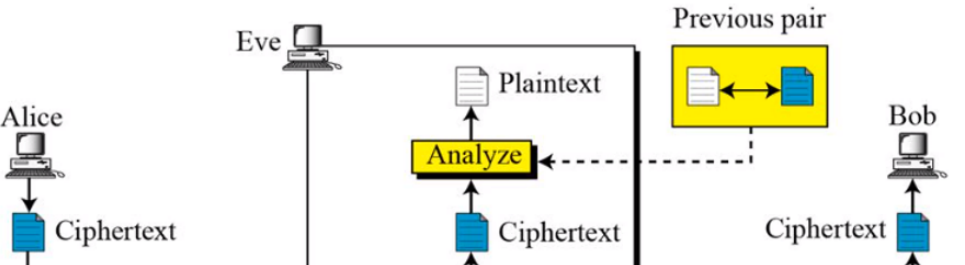
\includegraphics[width=105.63mm,height=73.06mm]{../../images/llm/page_008_img_01.png}%
\end{textblock*}

\end{document}
